\documentclass[border=3pt]{standalone}
% Preâmbulo compartilhado pelos diagramas TikZ da aula 14 (SLAM com EIF)
\usepackage[T1]{fontenc}
\usepackage[utf8]{inputenc}
\usepackage{lmodern}
\usepackage{amsmath}
\usepackage{xcolor}
\usepackage{tikz}
\usetikzlibrary{arrows.meta,angles,quotes,decorations.pathmorphing,decorations.pathreplacing,calc,
                positioning,shapes.geometric,shapes.misc,backgrounds,fit,
                math}

% Paleta (mesma dos SVGs originais)
\definecolor{dblue}{HTML}{2A5B8C}
\definecolor{dorange}{HTML}{B3541E}
\definecolor{dgreen}{HTML}{4A7C59}
\definecolor{dred}{HTML}{9C4B4B}
\definecolor{dcream}{HTML}{F4F1EA}
\definecolor{dshade}{HTML}{DDD7C9}

% Função gaussiana (não normalizada por padrão de escala visual)
\pgfmathdeclarefunction{gauss}{3}{%
  \pgfmathparse{1/(#3*sqrt(2*pi))*exp(-((#1-#2)^2)/(2*#3^2))}%
}

% Estilos comuns (prefixo d... para não colidir com chaves internas do pgf)
\tikzset{
  >={Stealth[length=2mm]},
  dguide/.style={gray!55, dashed, line width=0.4pt},
  daxis/.style={gray!60, line width=0.7pt, ->},
  dbody/.style={fill=black!3, draw=black!80, line width=1pt},
  dacc/.style={draw=dblue, line width=1pt},
  dlbl/.style={black!55, font=\small},
  dsub/.style={black!45, font=\footnotesize},
  dstate/.style={circle, draw=black!80, fill=dcream, line width=1pt,
                 minimum size=17mm, font=\large, inner sep=1pt},
  dobs/.style={circle, draw=black!80, fill=dshade, line width=1pt,
               minimum size=14mm, font=\large, inner sep=1pt},
  dbox/.style={rounded corners=2pt, draw=black!80, fill=dcream, line width=1pt,
               align=center, inner sep=6pt},
  dop/.style={circle, draw=black!80, fill=white, line width=1pt,
              minimum size=6mm, inner sep=0pt, font=\small},
  dtrans/.style={->, dblue, line width=1pt},
  dmeas/.style={->, dorange, line width=1pt},
  dcurve/.style={line width=1pt, dblue},
  dcurveb/.style={line width=1.4pt, dorange},
}

\begin{document}
\hyphenpenalty=10000 \exhyphenpenalty=10000 \tolerance=9999 \emergencystretch=3em
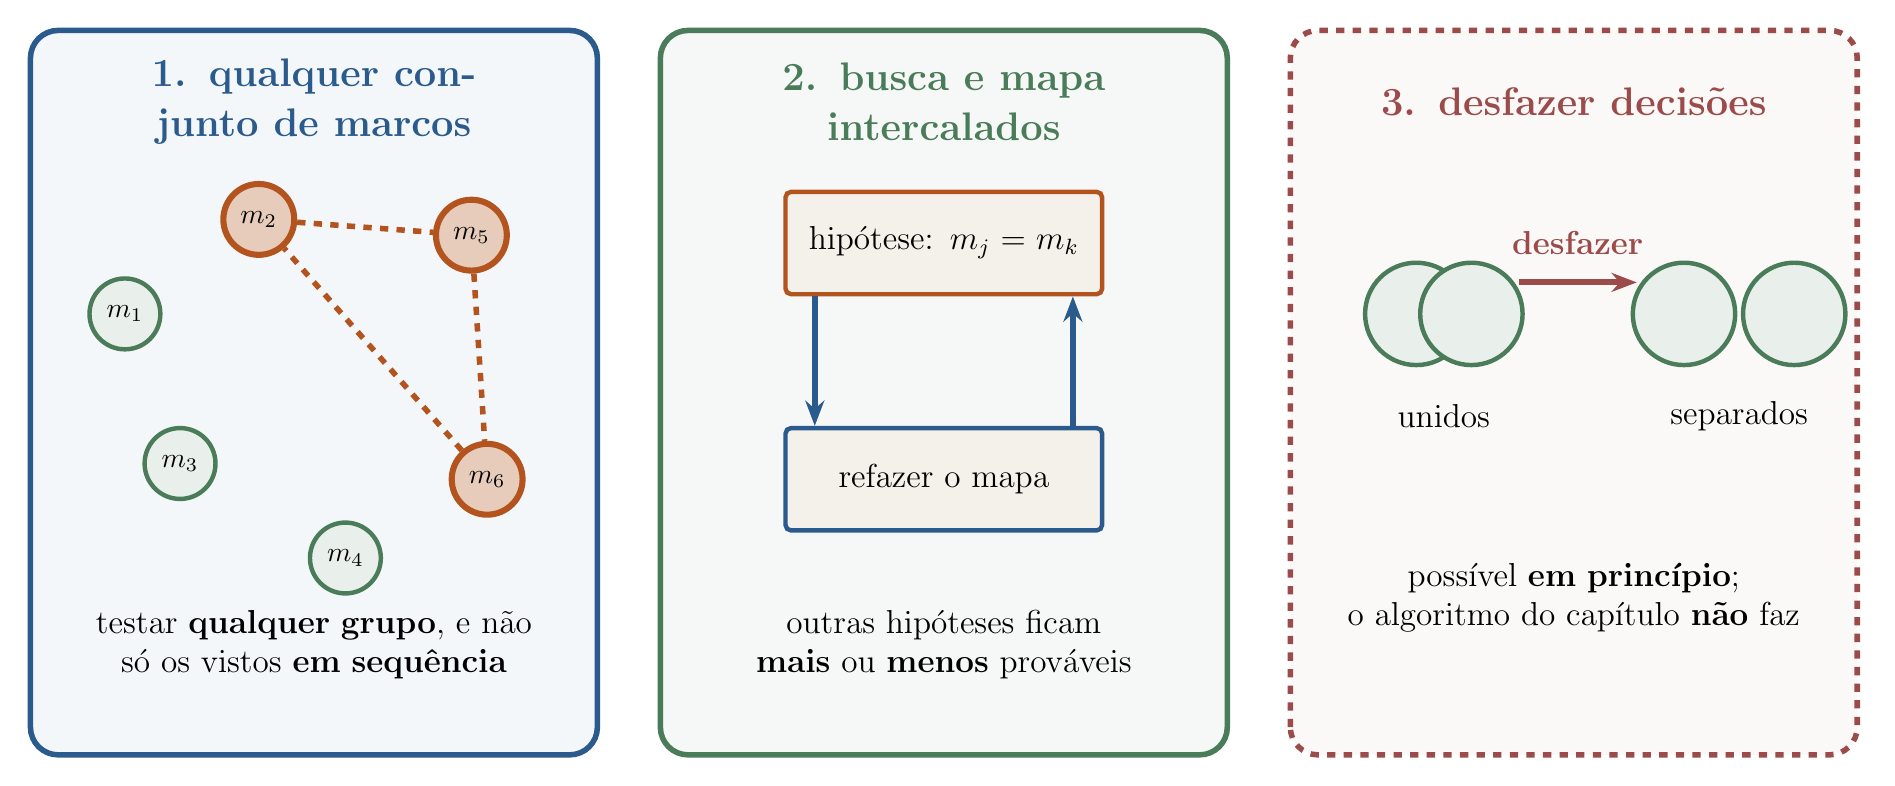
\begin{tikzpicture}[x=1cm,y=1cm]
\tikzset{m/.style={circle, draw=dgreen, fill=dgreen!12, line width=1.6pt, minimum size=0.9cm, font=\normalsize},
        s/.style={circle, draw=dorange, fill=dorange!30, line width=2.2pt, minimum size=0.9cm, font=\normalsize},
        k/.style={dbox, text width=3.6cm, minimum height=1.3cm, font=\large, line width=1.6pt}}
% painel 1
\draw[draw=dblue, line width=2pt, fill=dblue!5, rounded corners=10pt] (0,-0.6) rectangle (7.2,8.6);
\node[font=\Large\bfseries, text=dblue, text width=6.6cm, align=center] at (3.6,7.7) {1. qualquer conjunto de marcos};
\node[m] (a1) at (1.2,5.0) {$m_1$}; \node[s] (a2) at (2.9,6.2) {$m_2$}; \node[m] (a3) at (1.9,3.1) {$m_3$}; \node[m] (a4) at (4.0,1.9) {$m_4$};
\node[s] (a5) at (5.6,6.0) {$m_5$}; \node[s] (a6) at (5.8,2.9) {$m_6$};
\draw[dorange, dashed, line width=2pt] (a2) -- (a5) -- (a6) -- (a2);
\node[font=\large, text width=6.6cm, align=center] at (3.6,0.8) {testar \textbf{qualquer grupo}, e não só os vistos \textbf{em sequência}};
% painel 2
\draw[draw=dgreen, line width=2pt, fill=dgreen!5, rounded corners=10pt] (8.0,-0.6) rectangle (15.2,8.6);
\node[font=\Large\bfseries, text=dgreen, text width=6.6cm, align=center] at (11.6,7.7) {2. busca e mapa intercalados};
\node[k, draw=dorange] (h) at (11.6,5.9) {hipótese: $m_j=m_k$};
\node[k, draw=dblue] (r) at (11.6,2.9) {refazer o mapa};
\draw[dtrans, line width=2.2pt, -{Stealth[length=3.2mm]}] (h.south west) ++(0.4,0) -- ([xshift=0.4cm]r.north west);
\draw[dtrans, line width=2.2pt, -{Stealth[length=3.2mm]}] ([xshift=-0.4cm]r.north east) -- ([xshift=-0.4cm]h.south east);
\node[font=\large, text width=6.6cm, align=center] at (11.6,0.8) {outras hipóteses ficam \textbf{mais} ou \textbf{menos} prováveis};
% painel 3
\draw[draw=dred, dashed, line width=2pt, fill=dred!4, rounded corners=10pt] (16.0,-0.6) rectangle (23.2,8.6);
\node[font=\Large\bfseries, text=dred, text width=6.6cm, align=center] at (19.6,7.7) {3. desfazer decisões};
\node[m, minimum size=1.3cm] (u1) at (17.6,5.0) {}; \node[m, minimum size=1.3cm] (u2) at (18.3,5.0) {};
\node[font=\large, text width=3cm, align=center] at (17.95,3.7) {unidos};
\draw[dred, line width=2.2pt, -{Stealth[length=3.2mm]}] (18.9,5.4) -- (20.4,5.4); \node[font=\large\bfseries, text=dred] at (19.65,5.9) {desfazer};
\node[m, minimum size=1.3cm] (v1) at (21.0,5.0) {}; \node[m, minimum size=1.3cm] (v2) at (22.4,5.0) {};
\node[font=\large, text width=3cm, align=center] at (21.7,3.7) {separados};
\node[font=\large, text width=6.6cm, align=center] at (19.6,1.4) {possível \textbf{em princípio};\\ o algoritmo do capítulo \textbf{não} faz};
\end{tikzpicture}
\end{document}
